\documentclass{article}

\usepackage{fancyhdr} % Cabeceras de página
\usepackage{lastpage} % Módulo para añadir una referencia a la última página
\usepackage{titling} % No tengo claro para qué es esto
\usepackage[left=2cm,right=2cm,top=3cm,bottom=2cm]{geometry} % Márgenes
\usepackage{xspace}
\usepackage{graphicx}
\usepackage{tikz}
\usepackage{float}

\title{Optional Assignment 1}
\date{\today}
\author{SGNIP company}

\fancyhf{}
\fancypagestyle{plain}{%
	\lhead{\small \itshape \thetitle\, -\, \thedate\, -\, SEPRO}
	\rhead{\vspace{-20pt} 
\includegraphics[width=40 pt]{Logo.jpg}}
	\cfoot{\thepage\ of \pageref{LastPage}}
	\rfoot{}
}

\begin{document}

\maketitle

\section{Description}

We design the prototypes of a new interactive system for the Maximum hotel chain, specifically the interface that will be shown to the users on check-in and check-out, and in their room for requesting services and checking-out quickly. The system can be present in other public places in the hotel, such as bars or conference rooms.

The relationships between the different screens are shown below. After the relationship graph, each screen is shown at full size.

\newpage
\section{Relationship between screens}

\begin{figure}[H]
\centering
\begin{tikzpicture}

\node[label=above:{Figure \ref{figLanguages}}] (reception-in) at (0,0) {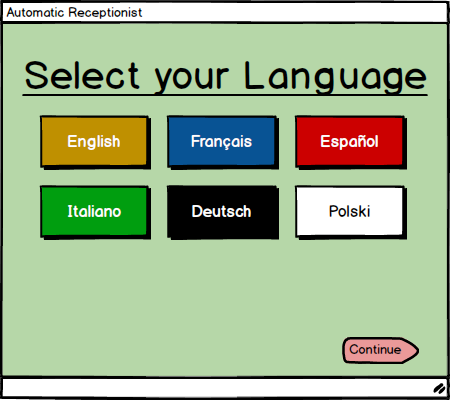
\includegraphics[width = 100pt]{Images/Base_1_Languages.png}};

\node[label=below:{Figure \ref{figCheckInOut}}] (check-in-out) at (5,-5) {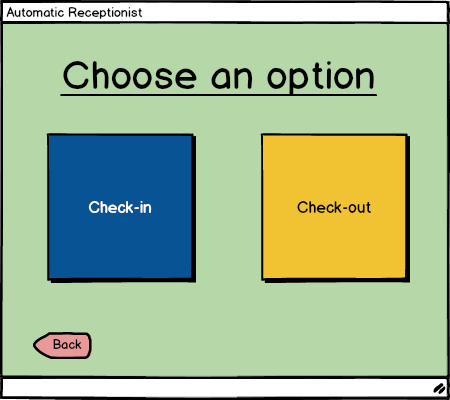
\includegraphics[width = 100pt]{Images/Basic_2_option.png}};
\node[label=below:{Figure \ref{figBarLogin}}] (bar-login) at (-5,-5) {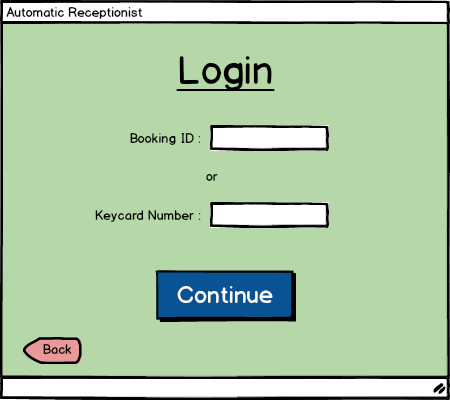
\includegraphics[width = 100pt]{Images/Services_2_Login.png}};
\node[label=below:{Figure \ref{figRoom}}] (room) at (0,-5) {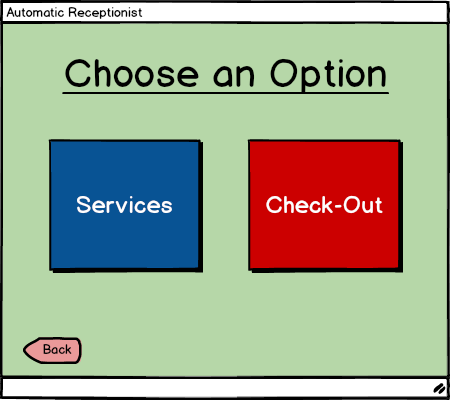
\includegraphics[width=100pt]{Images/Services_3_Selection.png}};

\node[label=below:{Figure \ref{figCheckIn}}] (check-in) at (5,-10) {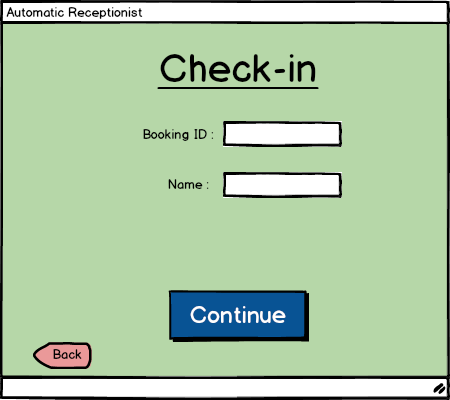
\includegraphics[width = 100pt]{Images/Basic_3_Check-in.png}};
\node[label=below:{Figure \ref{figServices}}] (services) at (-5,-10) {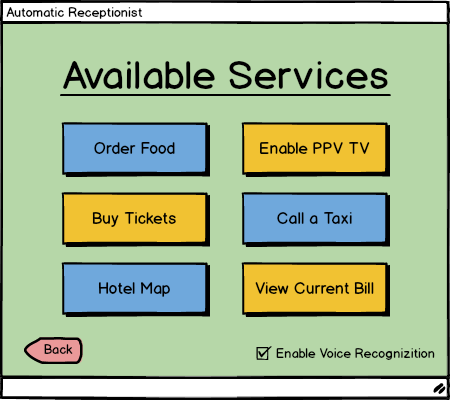
\includegraphics[width = 100pt]{Images/Services_4_Services.png}};
\node[label=below:{Figure \ref{figCheckOut}}] (check-out) at (0,-10) {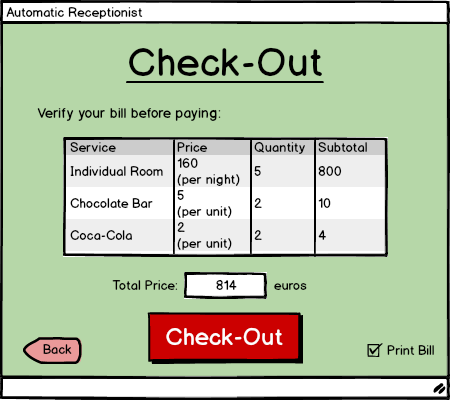
\includegraphics[width=100pt]{Images/Both_6_Check-Out.png}};

\node[label=below:{Figure \ref{figCheckInWrong}}] (check-in-wrong) at (6,-15) {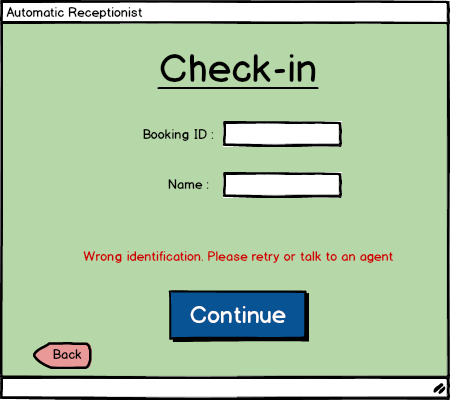
\includegraphics[width = 100pt]{Images/Basic_3_Check-in__wrong.png}};
\node[label=below:{Figure \ref{figServicesOrder}}] (services-order) at (-6,-15) {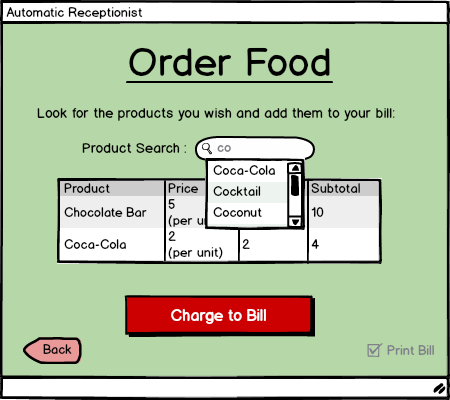
\includegraphics[width = 100pt]{Images/Services_5_Order-Food.png}};
\node[label=below:{Figure \ref{figGoodbye}}] (goodbye) at (-2,-15) {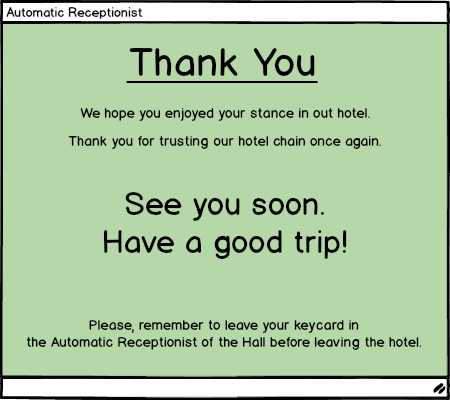
\includegraphics[width = 100pt]{Images/Both_7_Goodbye.png}};
\node[label=below:{Figure \ref{figCheckInDone}}] (check-in-done) at (2,-15) {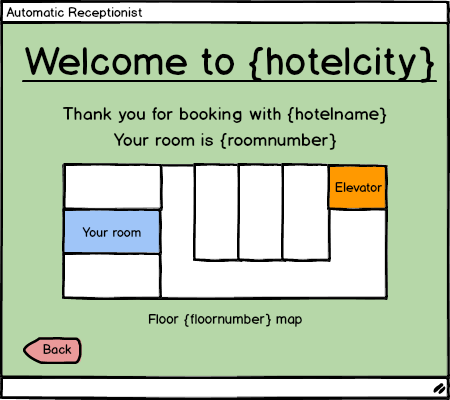
\includegraphics[width=100pt]{Images/Basic_4_CheckIn_Done.png}};

\draw[->] (reception-in) -- node[midway, above, sloped] {Reception} (check-in-out);
\draw[->] (reception-in) -- node[midway, above, sloped] {Public spaces} (bar-login);
\draw[->] (reception-in) -- node[midway, above, sloped] {Room} (room);

\draw[->] (bar-login) -- (services);
\draw[->] (room) -- (services);

\draw[->] (check-in-out) -- (check-out);
\draw[->] (room) -- (check-out);

\draw[->] (check-in-out) -- (check-in);

\draw[->] (services) -- (services-order);
\draw[->] (check-out) -- (goodbye);
\draw[->] (check-in) -- (check-in-done);
\draw[->] (check-in) -- node[midway, right, align=center] {Bad credentials} (check-in-wrong);



\end{tikzpicture}
\caption{Relationship between the screens.}
\end{figure}

\section{Detailed prototypes}

\subsection{Welcome screens}
\begin{figure}[H]
\centering
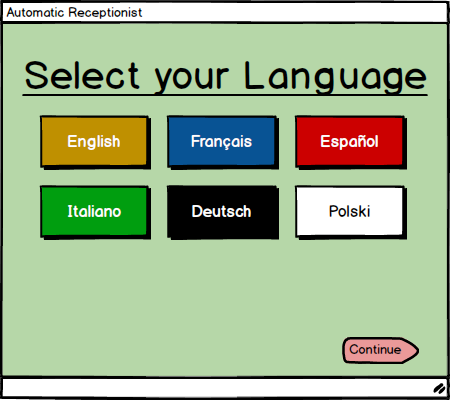
\includegraphics[width=0.6\textwidth]{Images/Base_1_Languages.png}
\caption{Language choosing screen.}
\label{figLanguages}
\end{figure}

\begin{figure}[H]
\centering
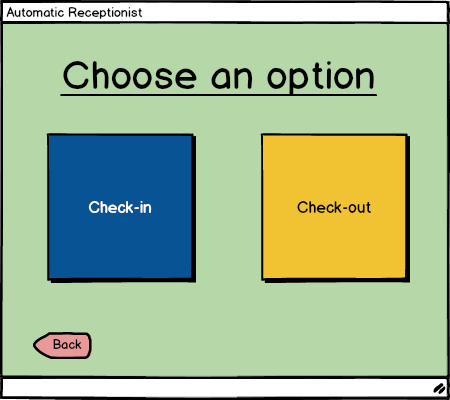
\includegraphics[width=0.6\textwidth]{Images/Basic_2_option.png}
\caption{Screen for choosing check-in or out.}
\label{figCheckInOut}
\end{figure}

\begin{figure}[H]
\centering
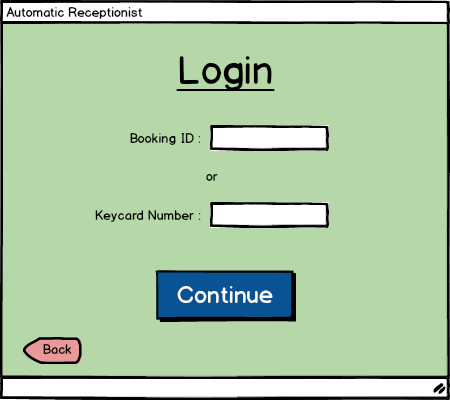
\includegraphics[width=0.6\textwidth]{Images/Services_2_Login.png}
\caption{Login screen for system points present in public places in the hotel other than the reception.}
\label{figBarLogin}
\end{figure}

\begin{figure}[H]
\centering
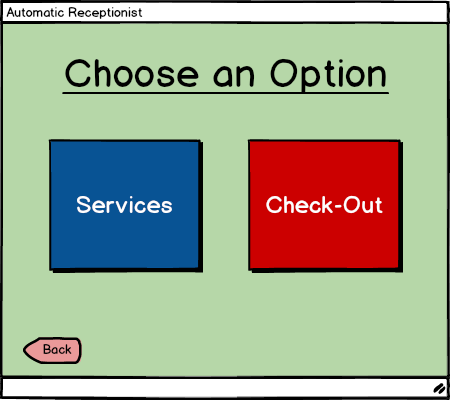
\includegraphics[width=0.6\textwidth]{Images/Services_3_Selection.png}
\caption{Screen for services or check-out, present in system points in user rooms.}
\label{figRoom}
\end{figure}

\subsection{Services}

\begin{figure}[H]
\centering
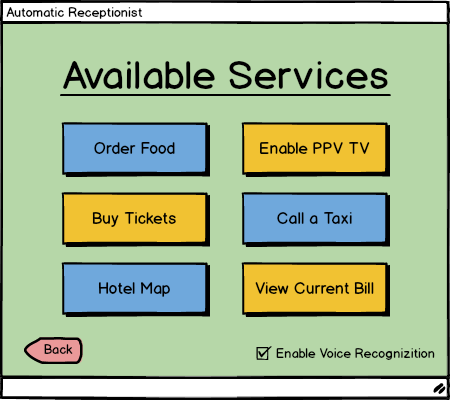
\includegraphics[width=0.6\textwidth]{Images/Services_4_Services.png}
\caption{Available services screen.}
\label{figServices}
\end{figure}


\begin{figure}[H]
\centering
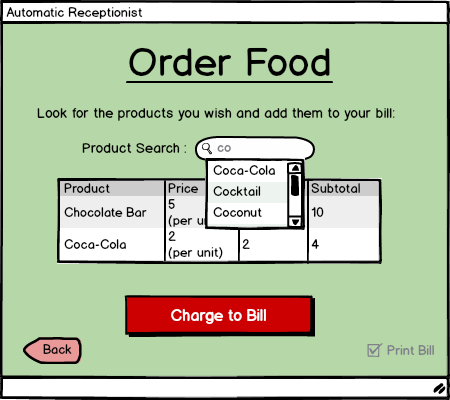
\includegraphics[width=0.6\textwidth]{Images/Services_5_Order-Food.png}
\caption{Sample screen for ordering a service (in this case, food).}
\label{figServicesOrder}
\end{figure}

\subsection{Check-in}

\begin{figure}[H]
\centering
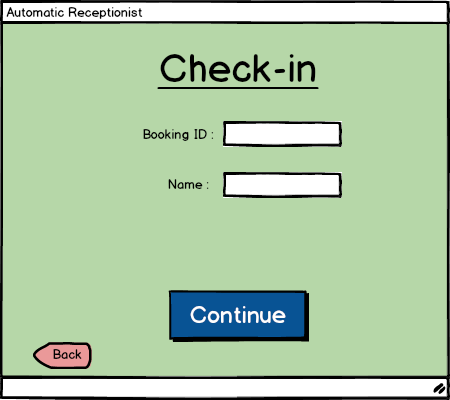
\includegraphics[width=0.6\textwidth]{Images/Basic_3_Check-in.png}
\caption{Check-in screen.}
\label{figCheckIn}
\end{figure}

\begin{figure}[H]
\centering
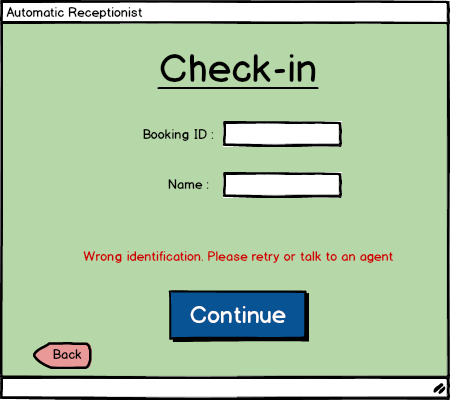
\includegraphics[width=0.6\textwidth]{Images/Basic_3_Check-in__wrong.png}
\caption{Error message shown when the check-in parameters are wrong.}
\label{figCheckInWrong}
\end{figure}

\begin{figure}[H]
\centering
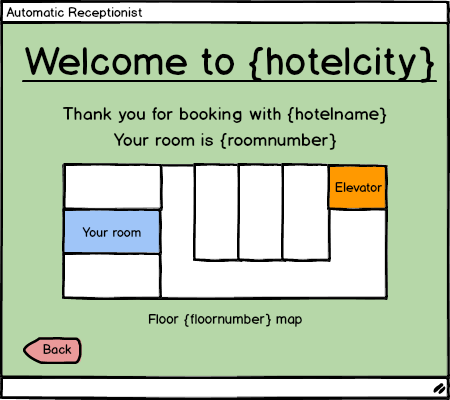
\includegraphics[width=0.6\textwidth]{Images/Basic_4_CheckIn_Done.png}
\caption{Welcome screen shown when the users checks in.}
\label{figCheckInDone}
\end{figure}

\subsection{Check-out}

\begin{figure}[H]
\centering
\includegraphics[width=0.6\textwidth]{Images/Both_6_Check-out.png}
\caption{Check-out screen.}
\label{figCheckOut}
\end{figure}


\begin{figure}[H]
\centering
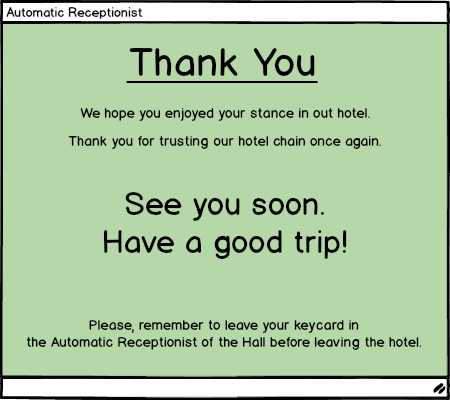
\includegraphics[width=0.6\textwidth]{Images/Both_7_Goodbye.png}
\caption{Goodbye screen for check-out.}
\label{figGoodbye}
\end{figure}

\end{document}
